\section{11. All Pairs Shortest Paths}

\begin{df}[APSP]
	Input: a graph $G(V, E)$ with a weight function $\\f : E \to [-u, u], \ |u| \leq |V|^{O(1)}$

	Output: matrix of shortest paths:
	\begin{align*}
		D \in \Z^{n \times n} : D[i, j] = \text{length between $i$ and $j$}
	\end{align*}

	Known: $O(n^3)$[Floyd, 1962]

	$O(n^3 / \log\log n)$

	$O(n^3 / \log n)$

	$O(n^3 / \log^2 n)$

	$O(n^3 / 2^{\sqrt{\log n}})$ [Williams, 2010](polynomial method)
\end{df}

\begin{df}[APSP Hypothesis]
	\begin{align*}
		\forall \varepsilon > 0, \text{APSP} \not \in n^{3 - \varepsilon}
	\end{align*}
\end{df}

\begin{df}[(min, +) - Matrix Multiplication]
	\label{df:matrix_multiplication_min_plus}
	Input: $A, B \in \Z^{n \times n}$

	Output: $C \in \Z^{n \times n}$:
	\begin{align*}
		C[i, j] = min_{k \in [n]} \ A[i, k] + B[k, j]
	\end{align*}

\end{df}

Matrix Multiplication(over $\Z$):
\begin{itemize}
	\item $O(n^3)$ naively
	\item $O(n^{\log_2 7}) = O(n^{2.8})$ [Strassen, 1969]

		\dots

	\item O(n^{2.37}) [Alman, Vassilevska Williams, 2011]
\end{itemize}

We also define $\omega = \inf \{ \alpha : MM \in \Ot(n^{\alpha}) \}$ (Matrix Multiplication exponent)

Conjecture: $\omega = 2$

(min, +) - Matrix Multiplication: it is subcubically equivalent to APSP, so we don't know how to solve it in $n^{3 - \varepsilon}$

Where Strassen's algorithm breaks down for (min, +)-Matrix Multiplication?

Strassen Alg:

\begin{figure}[ht]
	\centering
	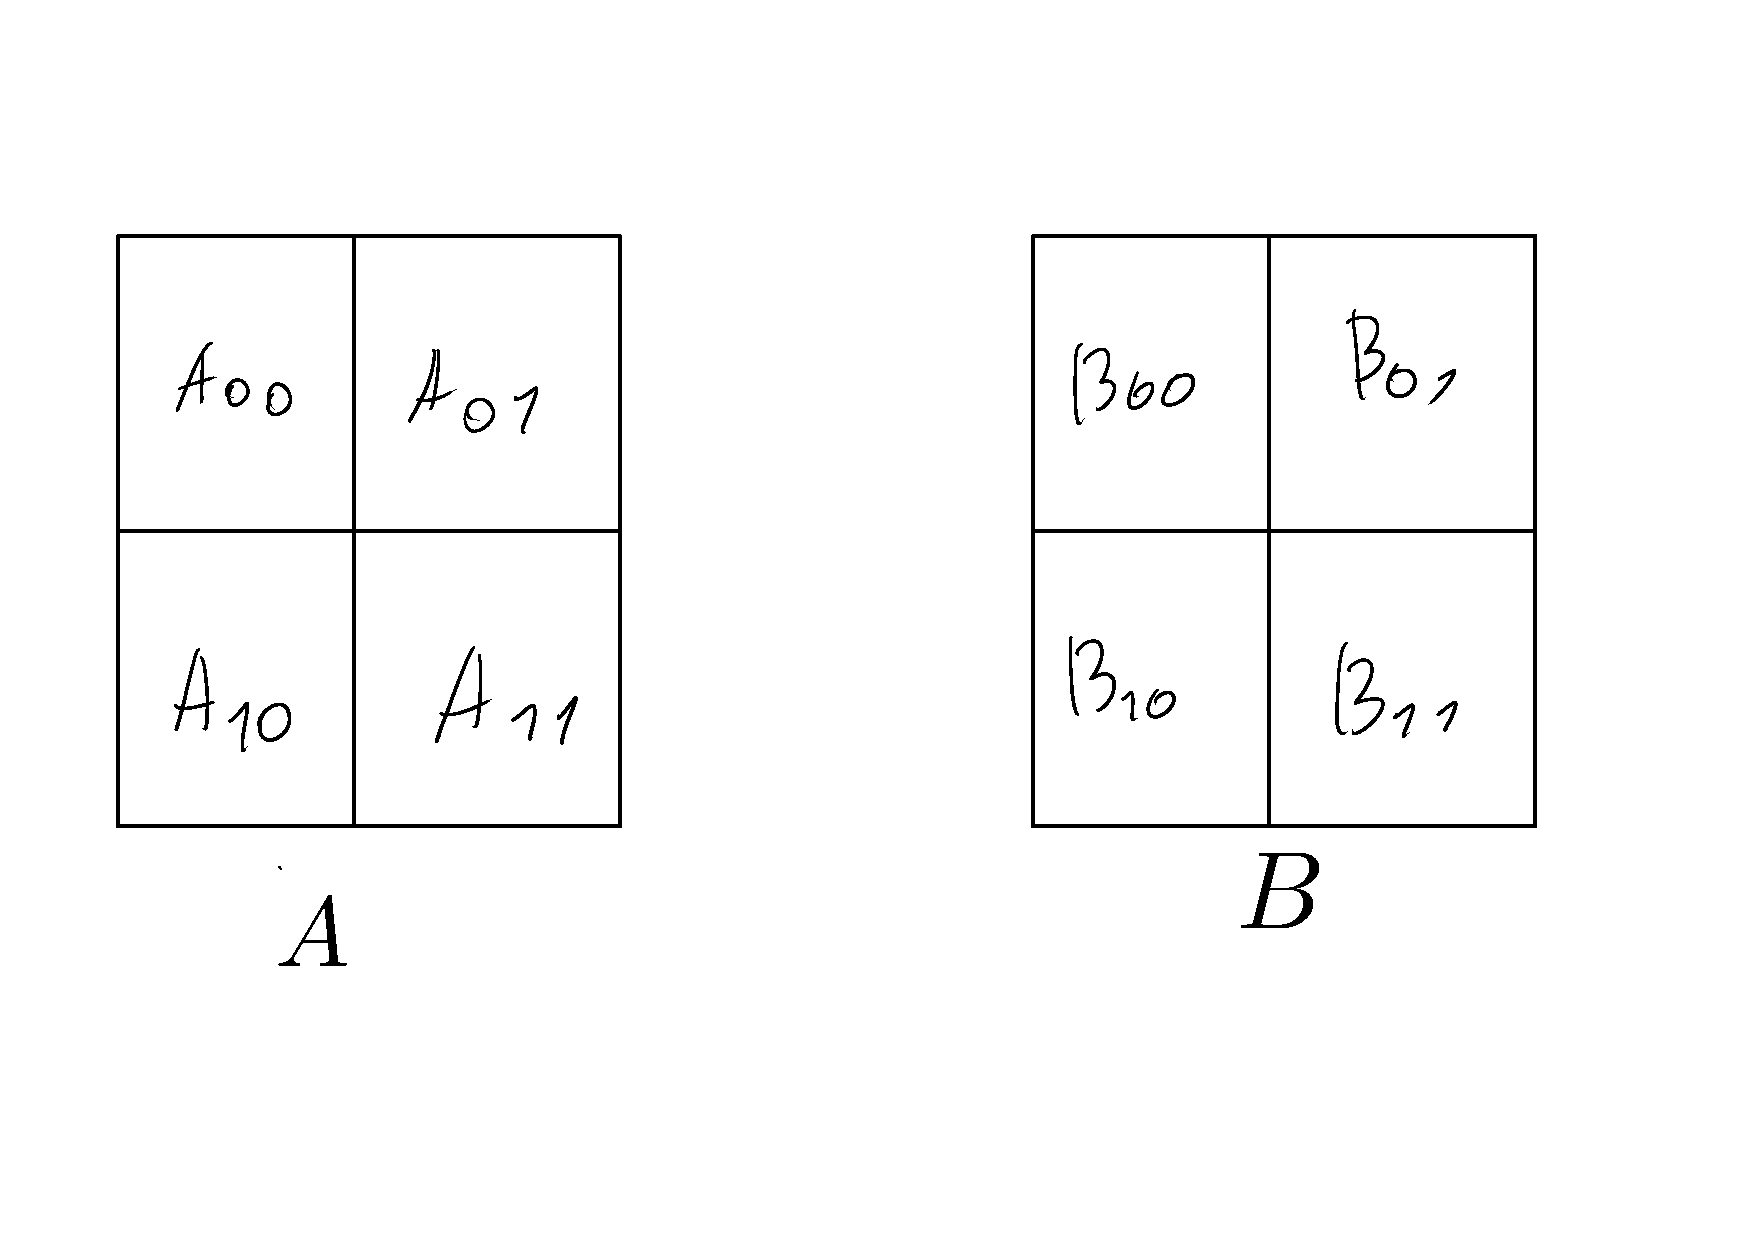
\includegraphics[scale=0.4]{figures/4.pdf}
	\caption{Strassen multiplication}
\end{figure}

Naively:
\begin{align*}
	T(n) \leq 8 T(\frac{n}{2}) + O(n^2) \Rightarrow T(n) = O(n^3)
\end{align*}

Strassen:

\begin{equation}
	\begin{cases}
		D_1 = (A_{00} + A_{01}) \cdot B_{01} \\
		D_2 = (A_{01} - A_{11}) \cdot (B_{10} - B({11})) \\
		\dots \\
		D_7 = \ldots
	\end{cases} \Rightarrow \text{$C_{00}, C_{01}, C_{10}, C_{11}$ linear comb. of $D_1 \dots D_7$  }
\end{equation}

Over $\Z$, "minus" is the inverse for "plus".
But for "min" there is no inverse!

\begin{df}[Triangle detection]
	Input: an unweight undirected graph $G(V, E)$.

	Output: is there a triangle in $G$? (Do there exists $i, j, k \in V : i \neq j, j \neq k, i \neq k$ and ${i, j}, {j, k}, {i, j} \in E$?  )

	Known: $O(n^3)$ - naively.

	$O(n^{1.5})$ for sparse graphs ($|E| = O(|V|)$ ) .

	$O(n^{\omega})$ $G$ contains a triangle $\Leftrightarrow A^3[i, i] > 0$ for some $i \in V$(because $A^k[i, j]$ is a count of $k$-walks from $i$ to $j$).

	\begin{figure}[ht]
		\centering
		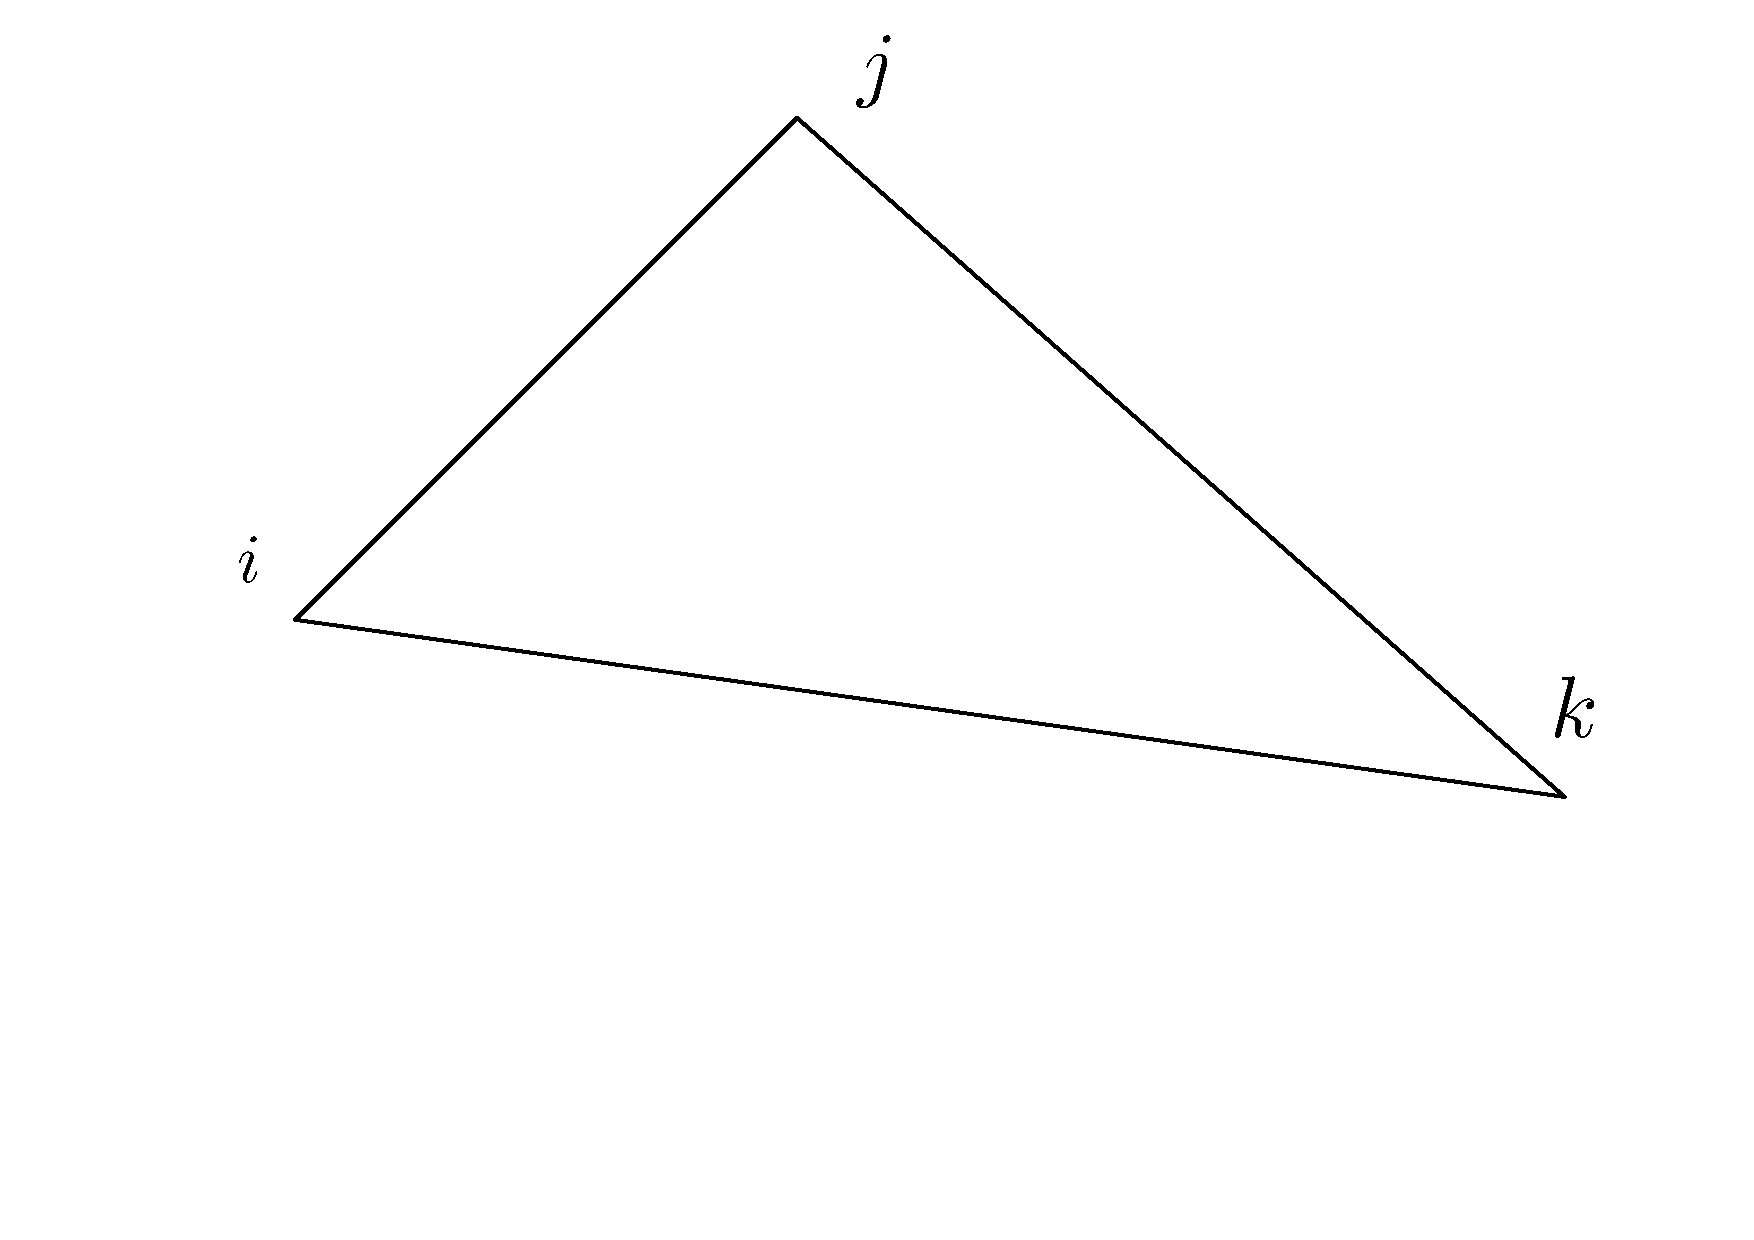
\includegraphics[scale=0.3]{figures/5.pdf}
		\caption{Triangle in a graph}
	\end{figure}
\end{df}

\begin{df}[Negative Triangle]
	\label{df:negative_triangle}
	Input: an undirected weighted $G(V, E)$.

	Output: is there a triangle with negative weight?
\end{df}

\begin{df}[Minimum Weight Triangle]
	Input: an undirected weighted $G(V, E)$.

	Output: triangle of minimum weight
\end{df}

\begin{df}[Zero Weight Triangle]
	Input: an undirected weighted $G(V, E)$.

	Output: is there a triangle with zero weight?
\end{df}

\begin{figure}[ht]
	\centering
	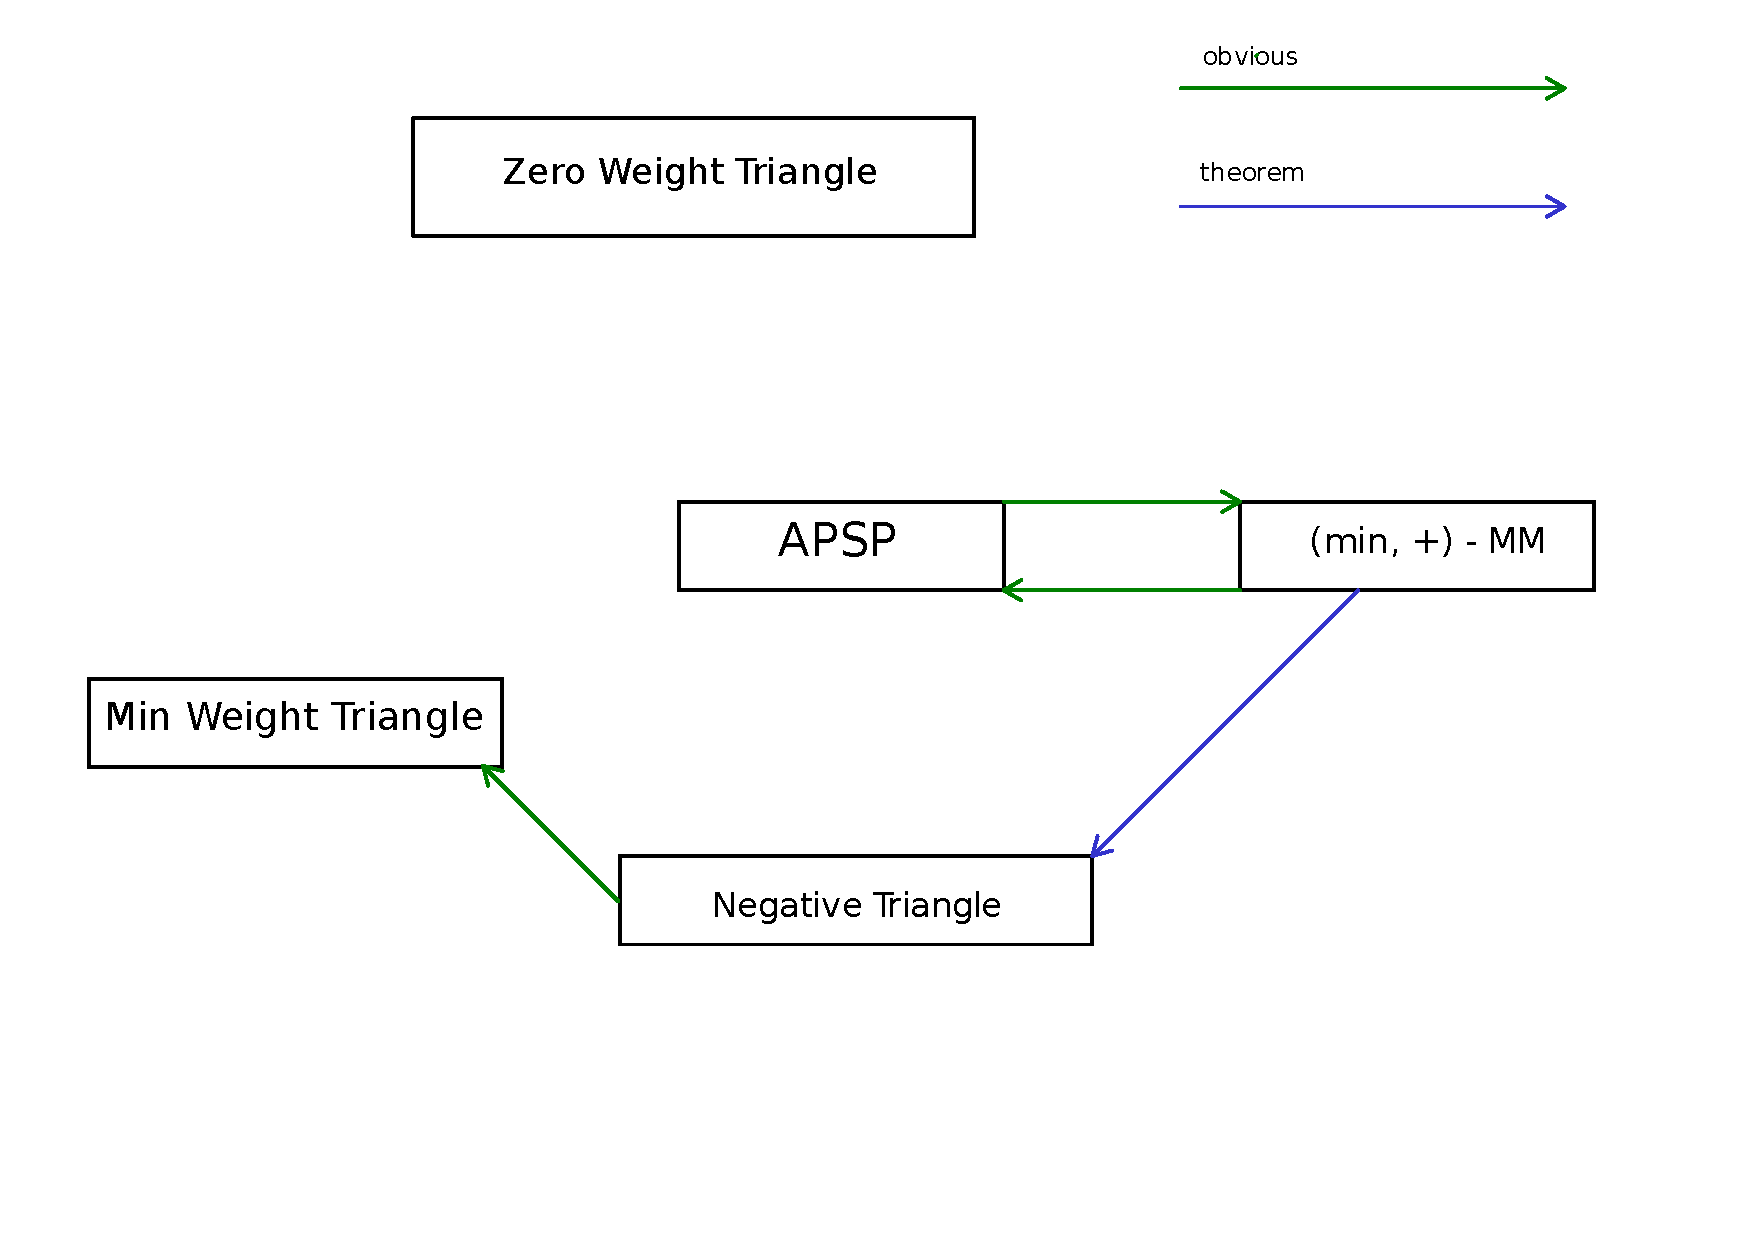
\includegraphics[scale=0.3]{figures/6.pdf}
	\caption{Reductions}
\end{figure}

\begin{thm}[Vassilevska-Williams, 2010]
	(min, +)-MM \eqref{df:matrix_multiplication_min_plus} reduces to Negative Triangle \eqref{df:negative_triangle}: if NegTri $\in n^{3 - \varepsilon}$, then (min, +)-MM $\in n^{3 - \sigma}$
\end{thm}

\begin{df}[All Pairs Negative Triangles]
	Input: tripartite weighted graph $G(I \sqcup J \sqcup K, E)$, $E \subseteq I \times J \cup I \times K \cup J \times K$
	\begin{figure}[ht]
		\centering
		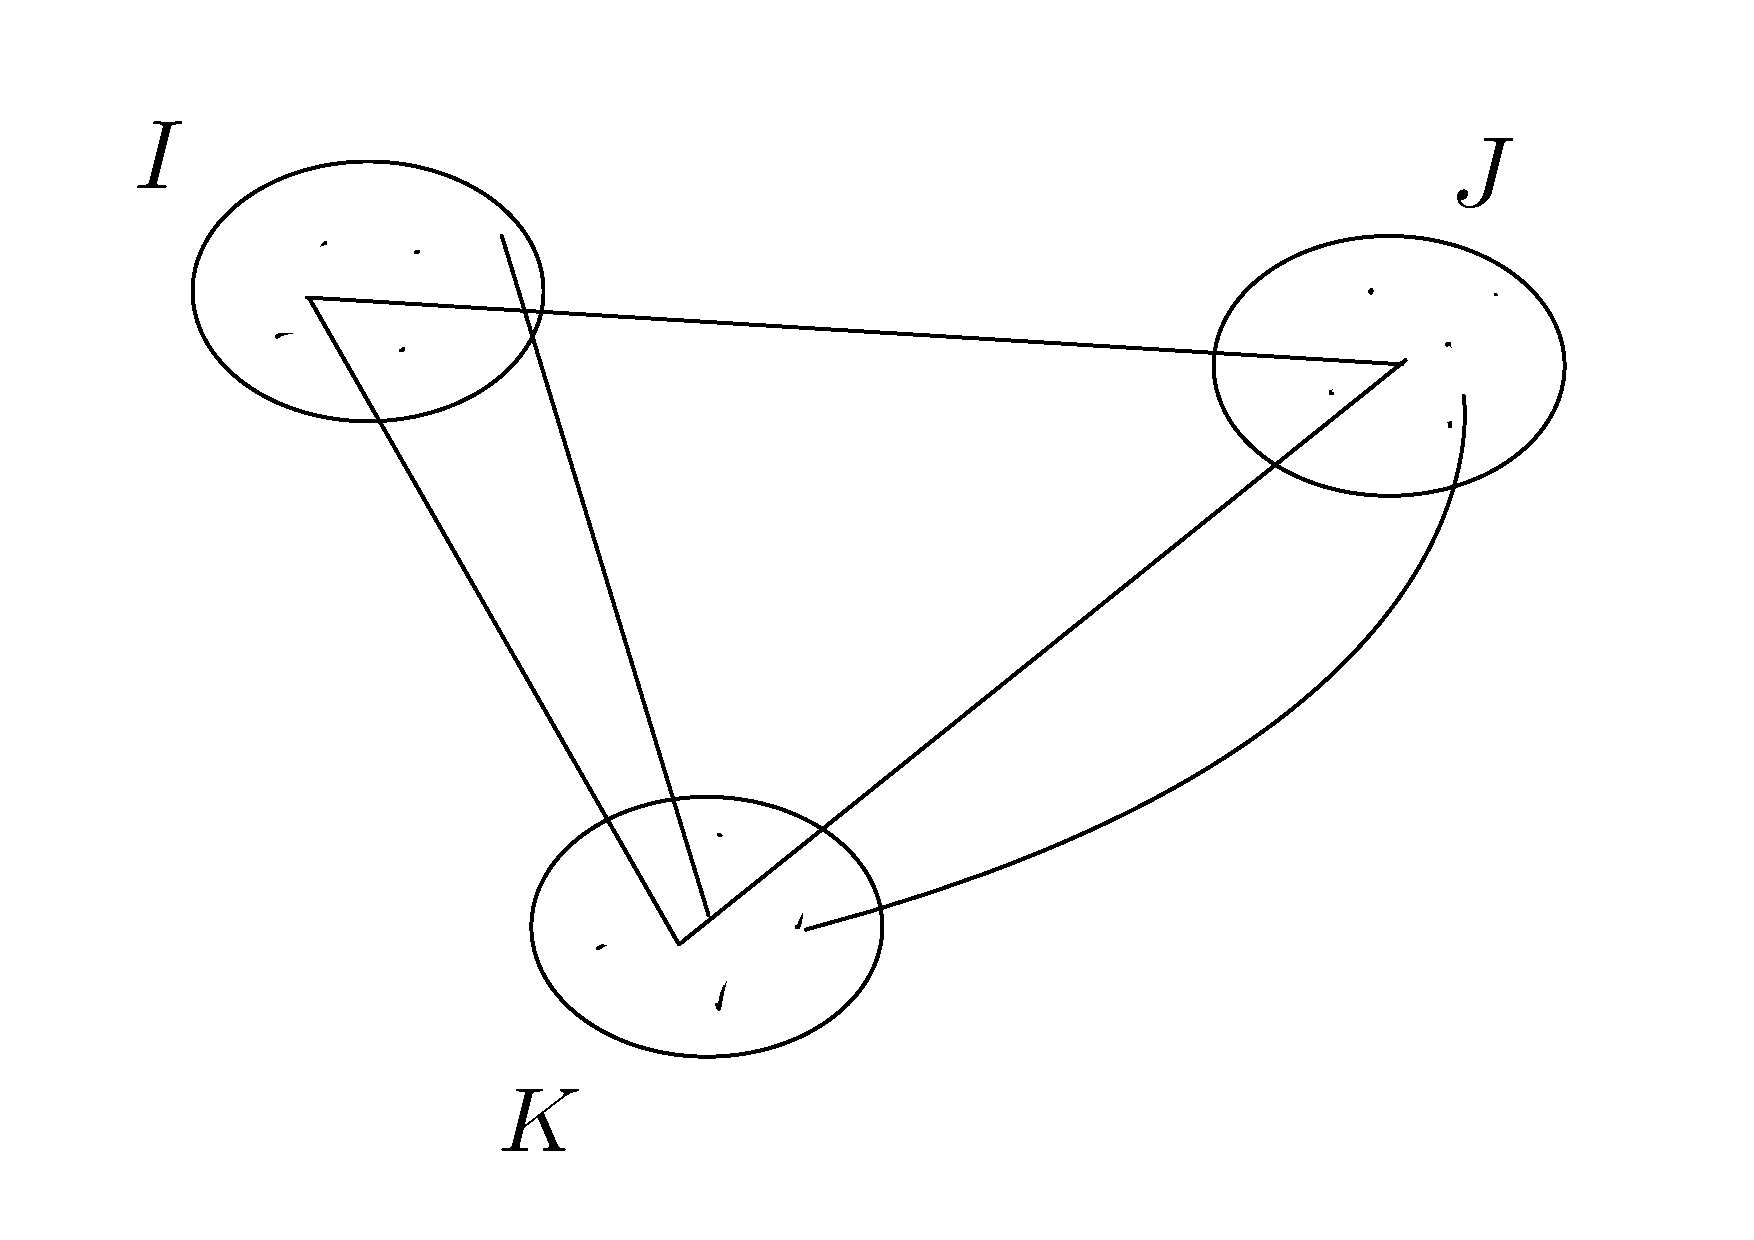
\includegraphics[scale=0.3]{figures/7.pdf}
		\caption{Thripartite}
	\end{figure}
	Output: $D \in \{0, 1\}^{n \times n}, D[i, j] = 1 \Leftrightarrow \exists k \in K : w(\triangle(i, j, k)) < 0$
	\begin{figure}[ht]
		\centering
		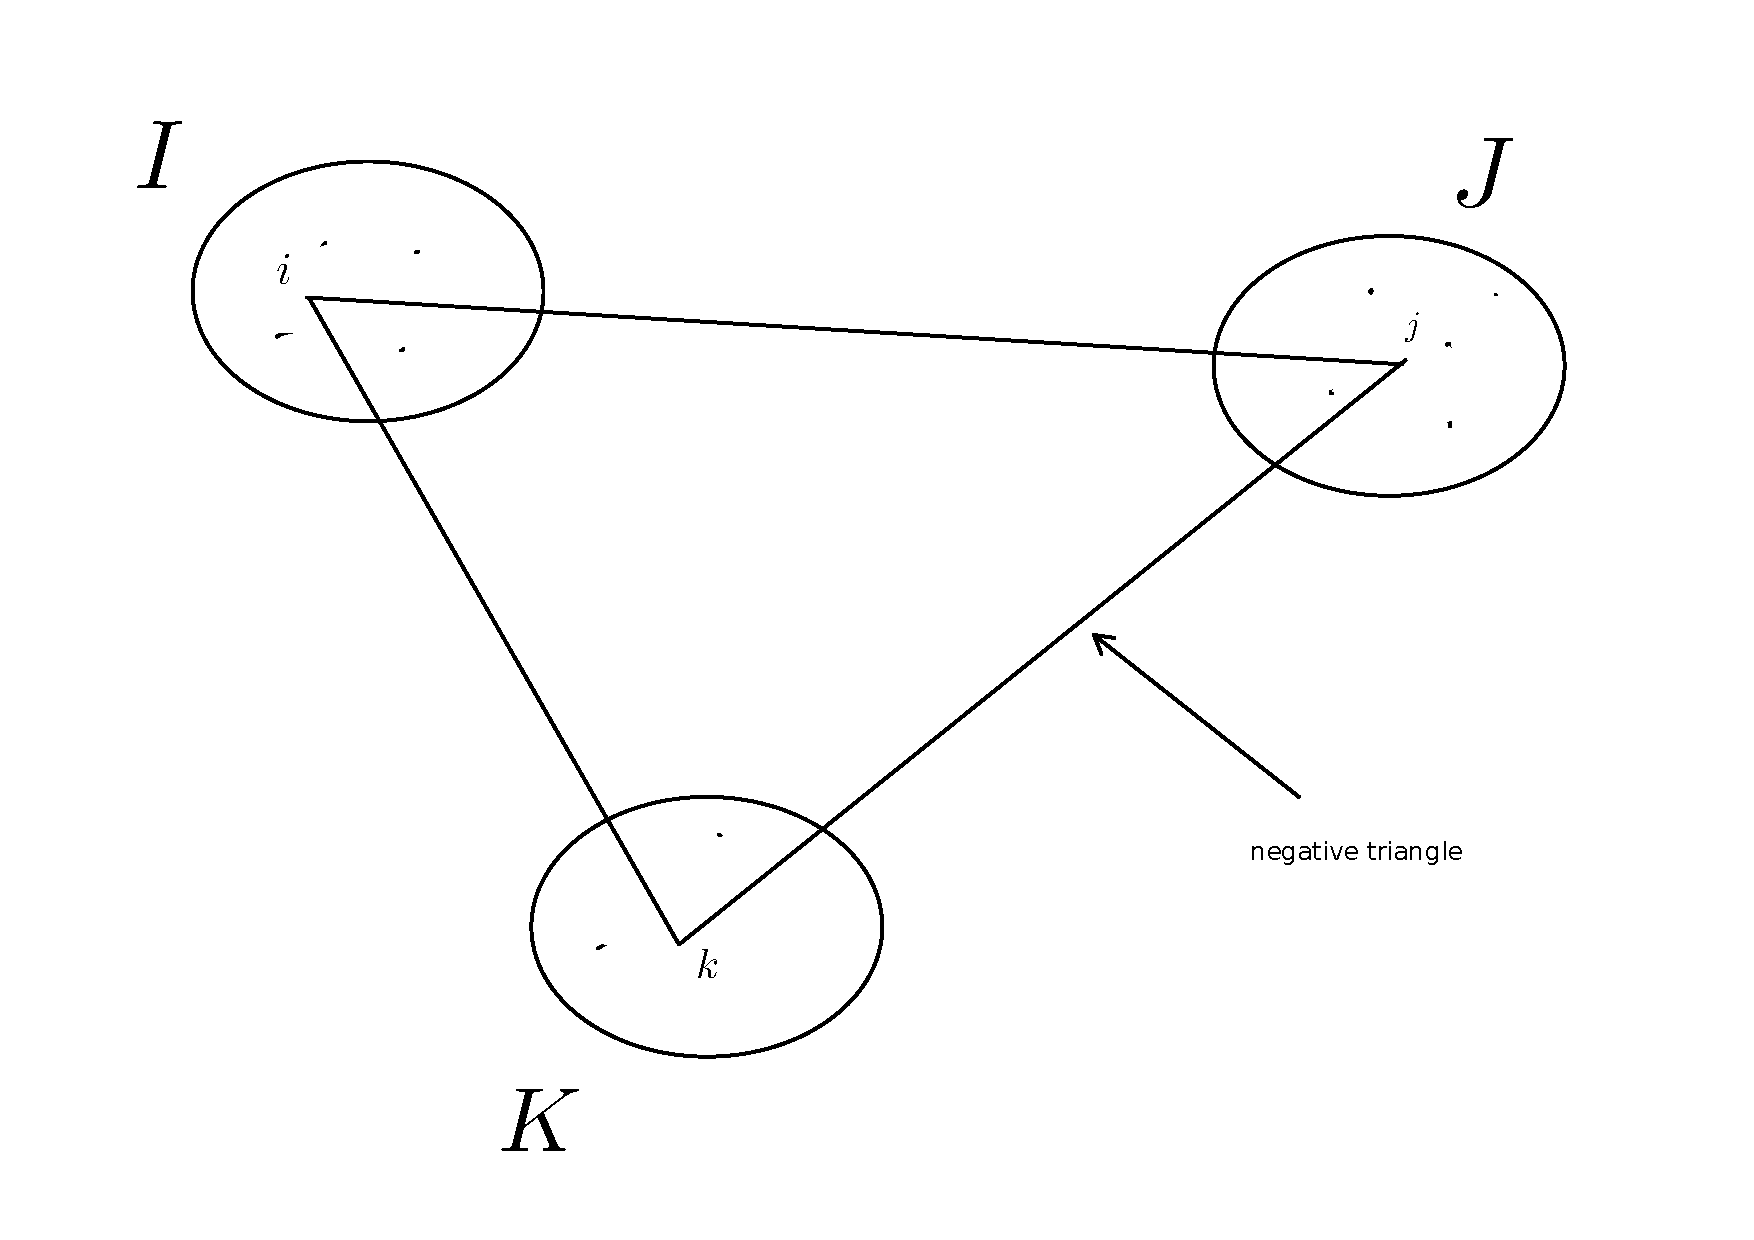
\includegraphics[scale=0.3]{figures/8.pdf}
		\caption{Negative triangle}
	\end{figure}
\end{df}

\begin{proof}
	Plan: (min, +)-MM $\to$ All Pairs Negative Triangles $\to$ Negative Triangle

	First reduction: (min, +)-MM $\to$ All Pairs Negative Triangle.

	\begin{align*}
		C[i, j] = \min_{k \in [n]} A[i, k] + B[k, j]
	\end{align*}
	\begin{figure}[ht]
		\centering
		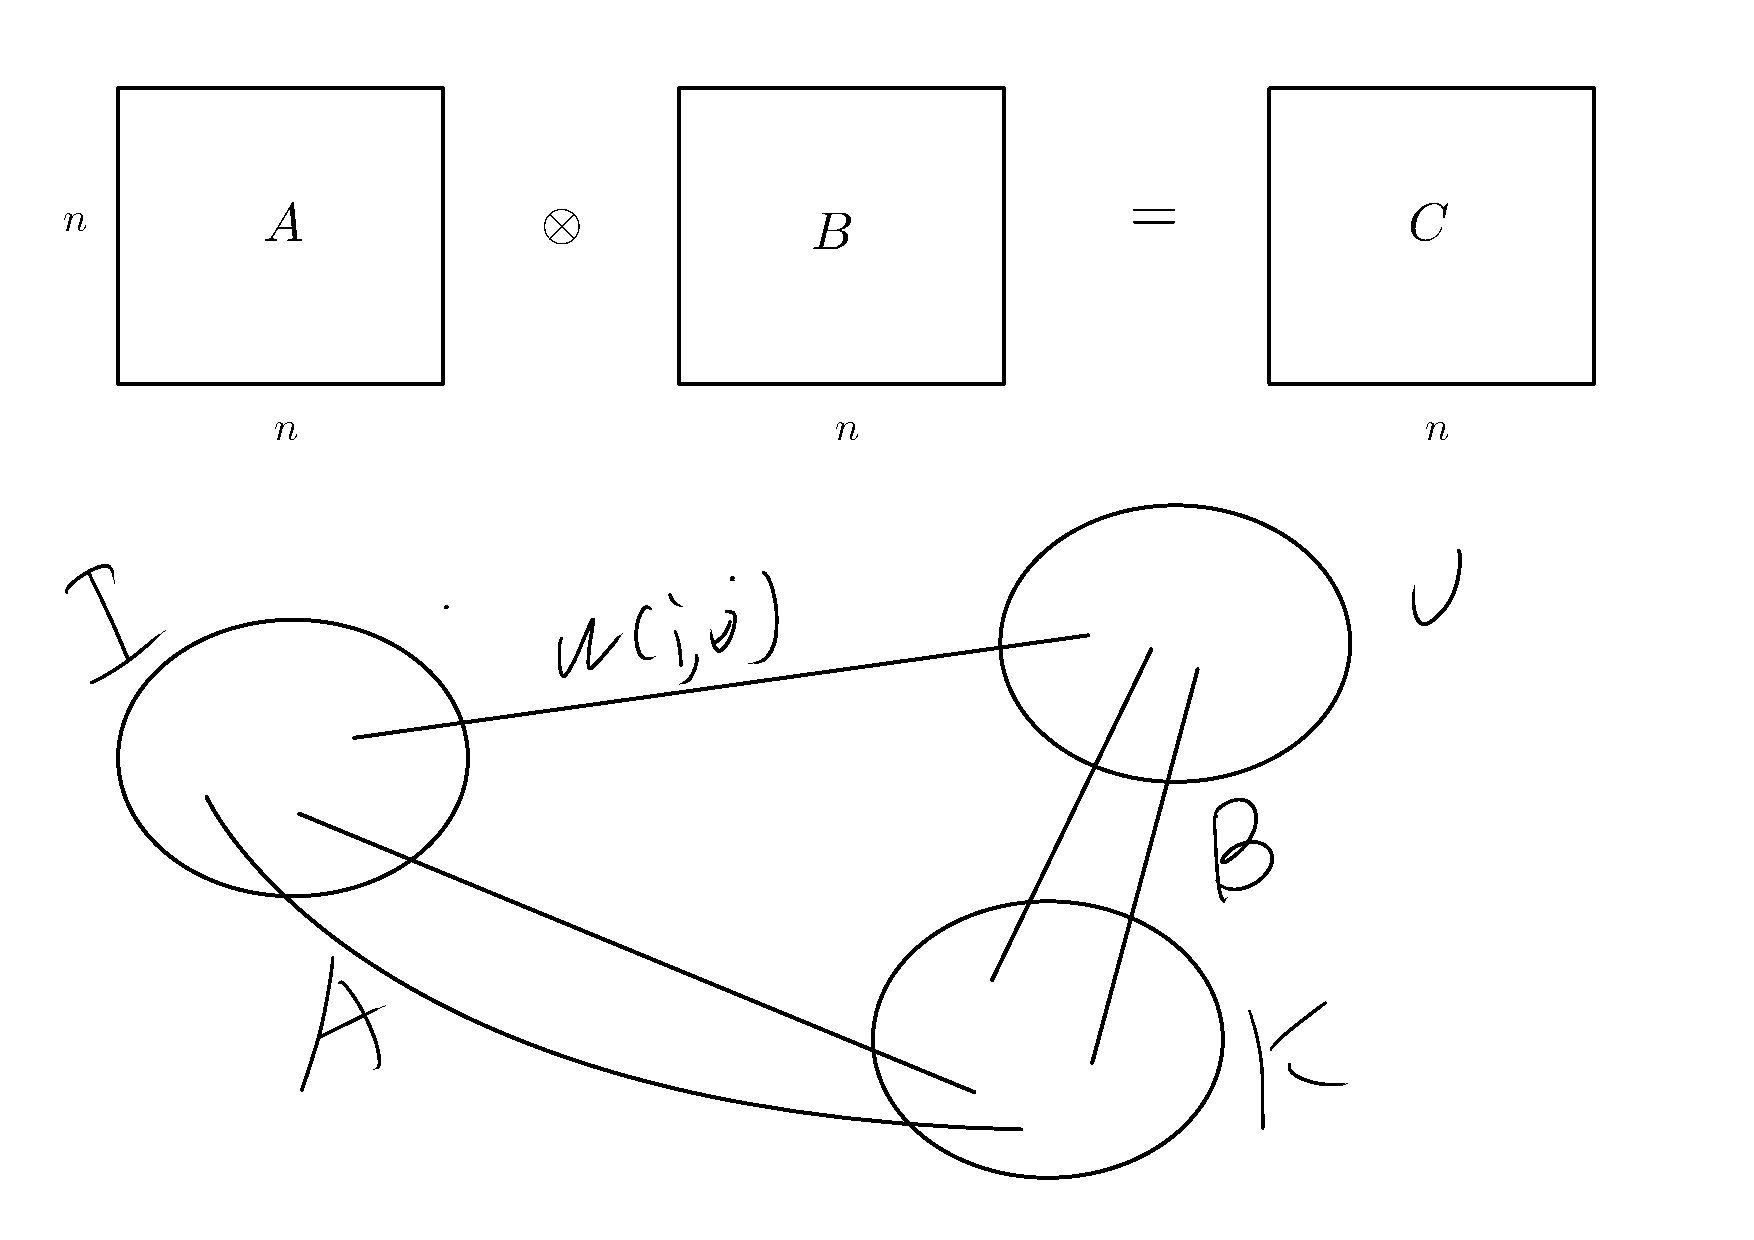
\includegraphics[scale=0.3]{figures/9.pdf}
		\caption{Constructing matrices $A, B$ }
	\end{figure}
	the edge $(i, j)$ participated in a negative triangle if $w(i, j) + C[i, j]$ < 0.

	Idea: simultaneous binary search: for every pair $(i, j)$ we find the largest value $t$ such that $t + c$ if $w(i ,j) = t$ then $(i, j)$ participates in a negative triangle.

	Then $C[i, j] = -t$
	\begin{figure}[ht]
		\centering
		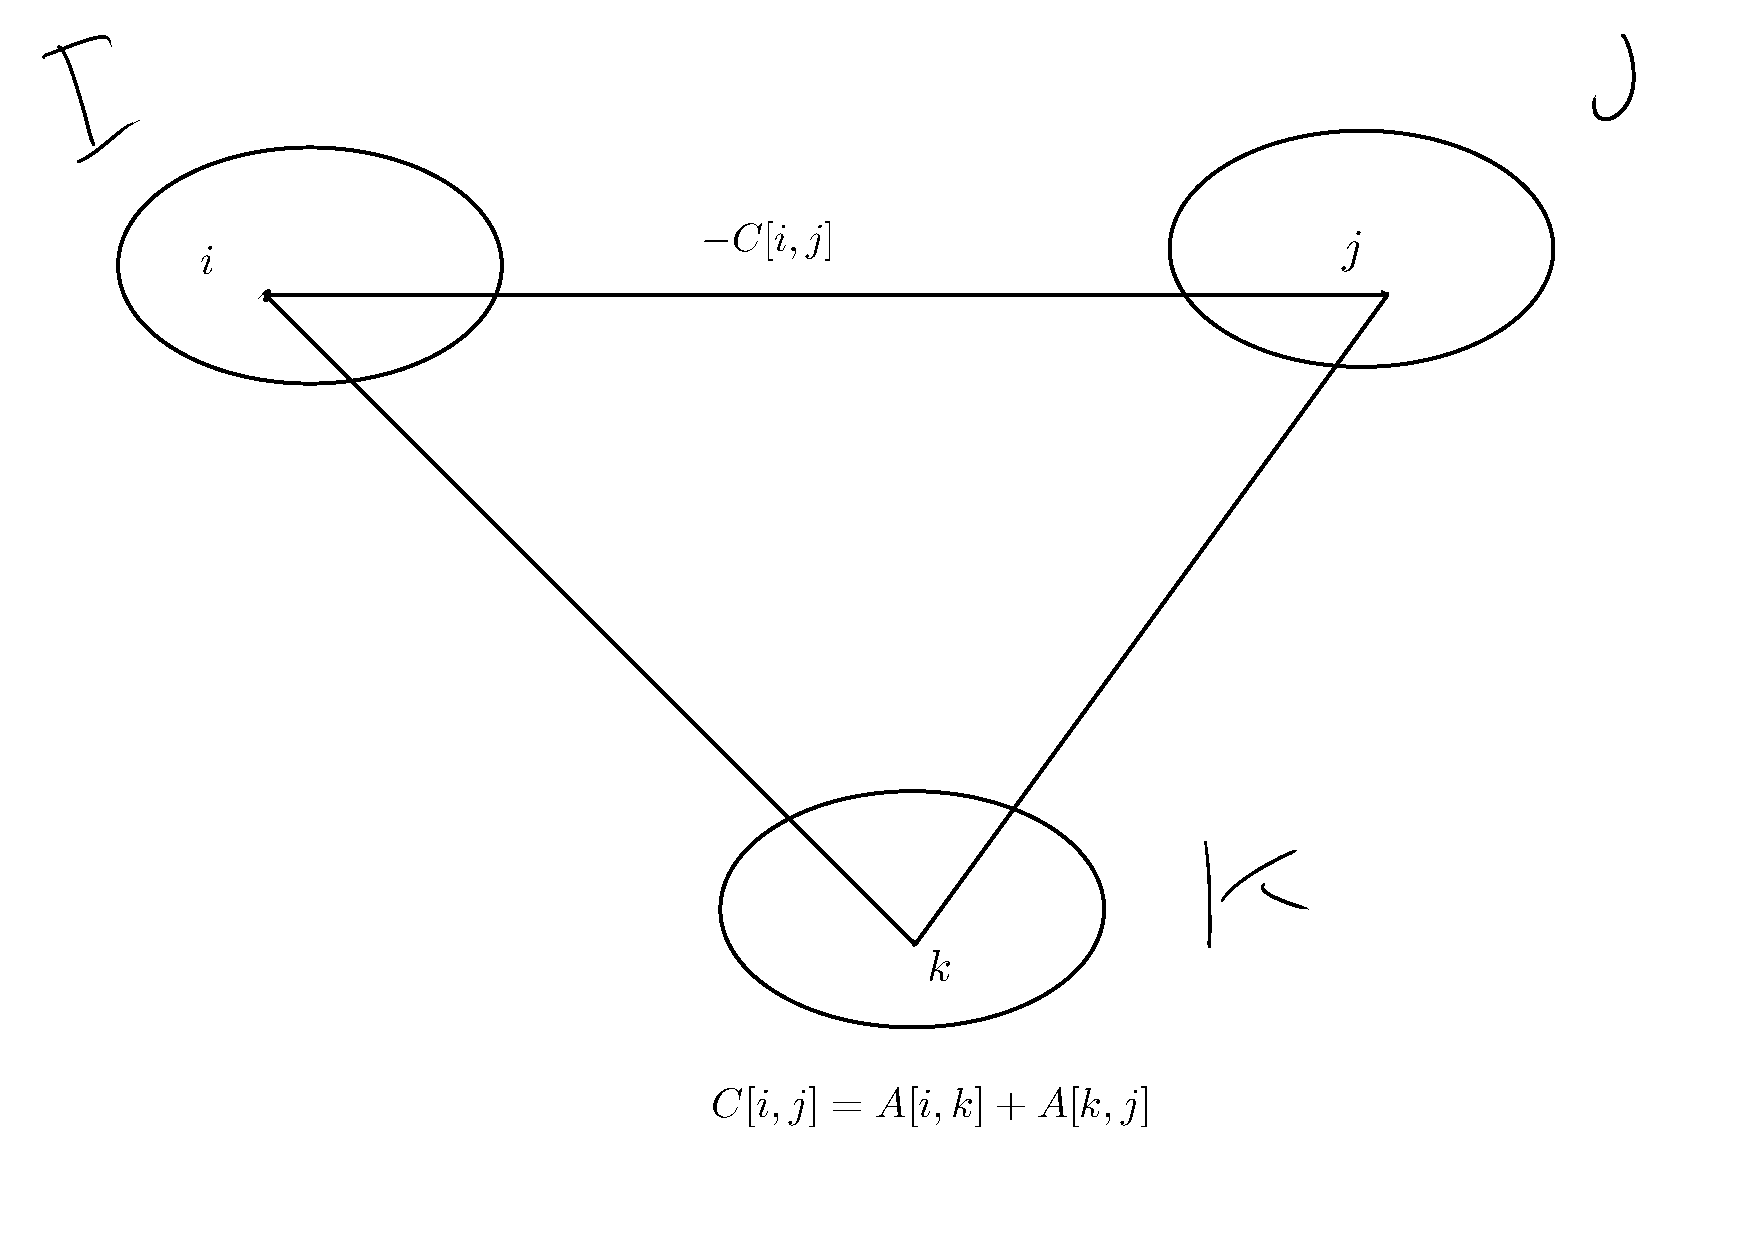
\includegraphics[scale=0.3]{figures/10.pdf}
		\caption{Representing idea}
	\end{figure}

	It completes reduction (min, +)-MM $\to$ All Pairs Negative Triangles.

	Now we will make a reduction from All Pairs Negative Triangles $\to$ Negative Triangle.

	Black box: Negative Triangle - assume (almost without loss of generality) that if solves the finding (rather than decision) version (similar: 3-SUM Finding -> 3-SUM).

	\begin{figure}[ht]
		\centering
		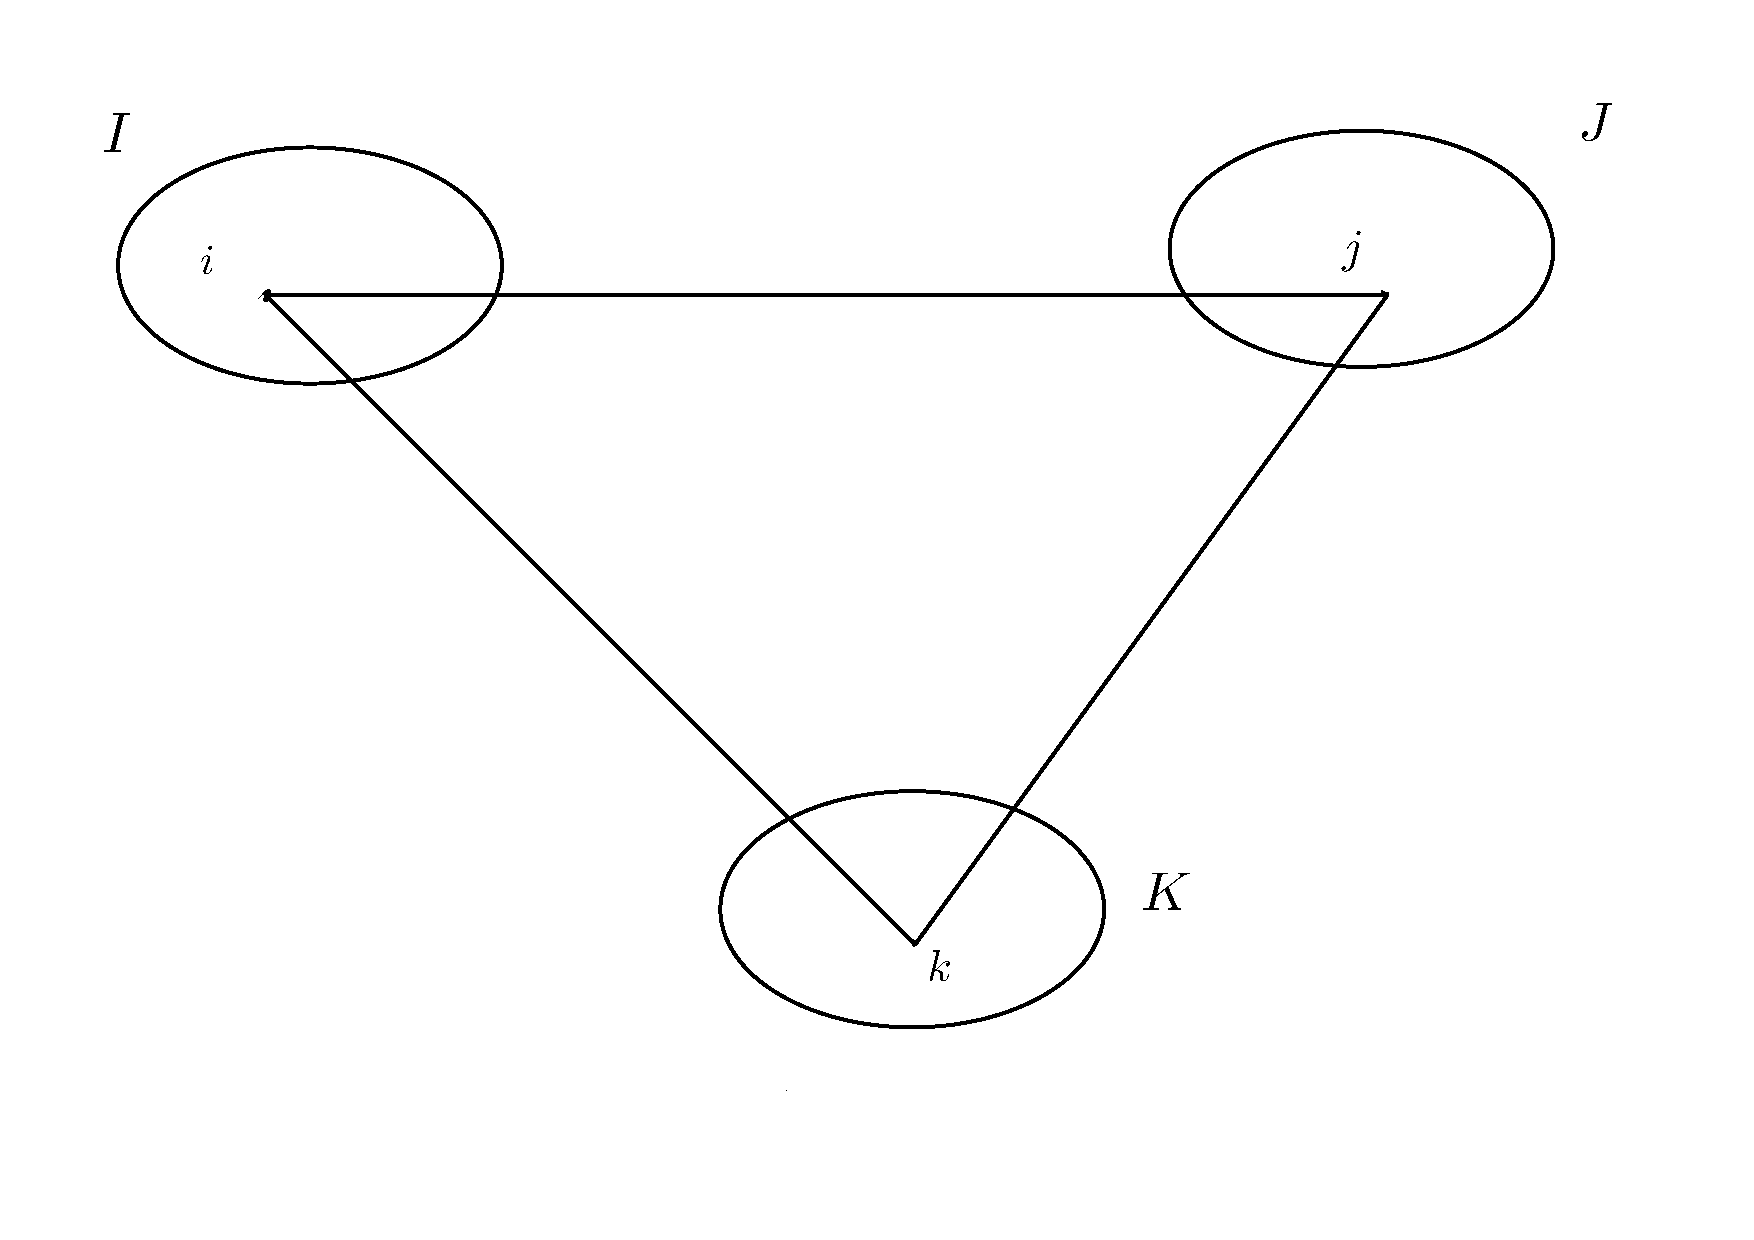
\includegraphics[scale=0.3]{figures/11.pdf}
		\caption{Negative triangle}
	\end{figure}

	? for every $i \in I, j \in J$ check whether $\exists k \in K : w(\triangle(i, j, k)) < 0$




	Partiion each of $I, J, K$ into $\frac{n}{s}$ parts of size $s$: $I = I_1 \sqcup \dots \sqcup I_{n / s}, J = \dots, K = \dots$

	Picture: \eqref{pic:thm_APNT_to_NT}

	\begin{figure}[ht]
		\centering
		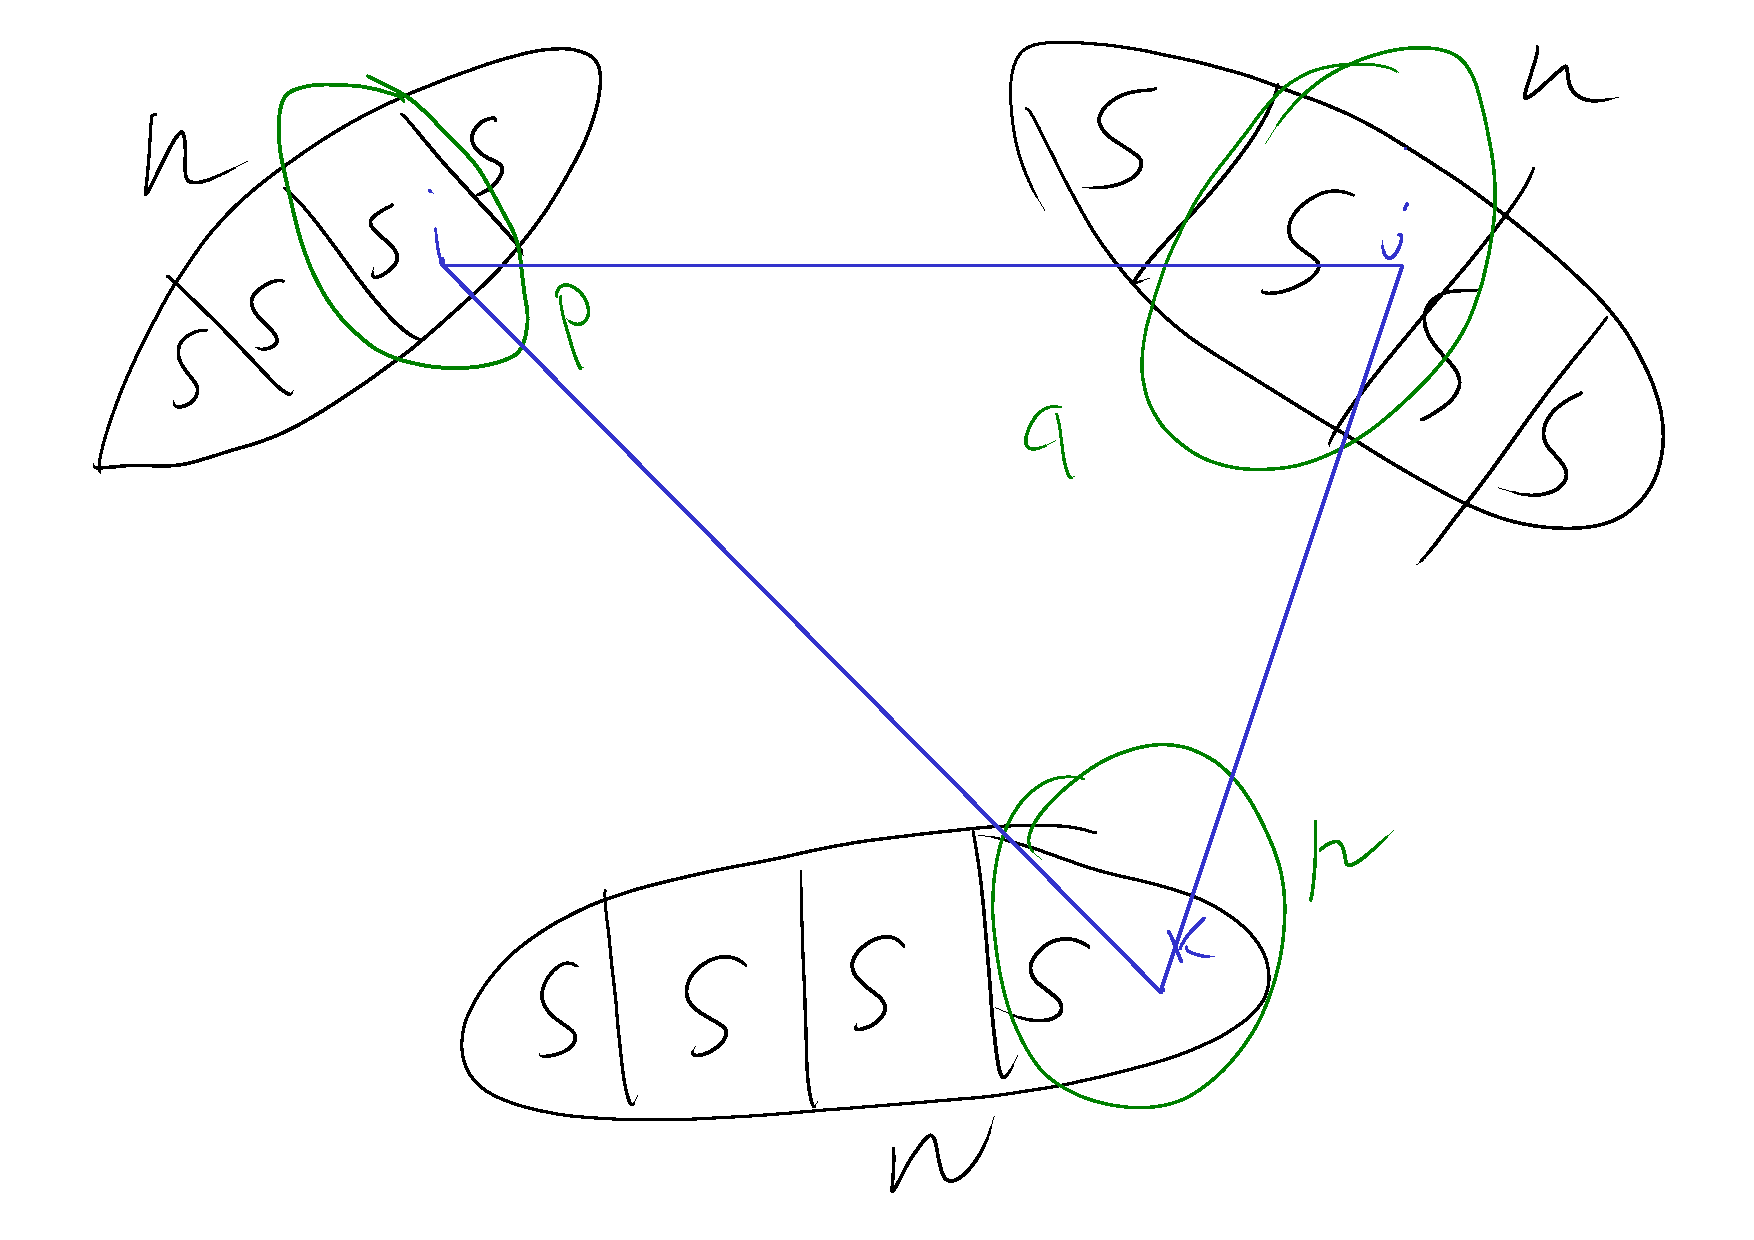
\includegraphics[scale=0.3]{figures/12.pdf}
		\caption{Partition}
		\label{pic:thm_APNT_to_NT}
	\end{figure}

	\begin{lstlisting}
$D \gets [0]^{n \times n}$
for all $1 \leq p, q, r \leq \frac{n}{s}$:
  while NegTriangle($G[I_p \sqcup J_q \sqcup K_r]$) = (i, j, k)
	# where $G[U]$ is a graph inducted by $U \subseteq V$
	$D[i, j] \gets 1$
	$w(i, j) \gets +\infty$
	\end{lstlisting}

	Assume that Negative Triangle $\in n^{3 - \varepsilon}$.

	Running time:

	\begin{align*}
		\underbrace{\text{\# calls of NegTriangle }}_{\leq (\frac{n}{s})^3 + n^2} \cdot s^{3 - \varepsilon} =
	\end{align*}

	Where $(\frac{n}{s})^3$ is a first calls and $n^2$ is a number of "successful" calls

	\begin{align*}
		=\left((\frac{n}{s})^3 + n^2\right) \cdot s^{3 - \varepsilon} = [(\frac{n}{s})^3 = n^2 \Leftrightarrow n =s^3 \Leftrightarrow s=\sqrt[3]{n}] = O(n^2 \cdot n^{\frac{3 - \varepsilon}{3}}) = O(n^{3 - \frac{\varepsilon}{3}})
	\end{align*}



\end{proof}
